\documentclass[9pt, aspectratio=169]{beamer}    %  presentation mode

\newcommand\titlebackgroundimage{fig/Marthe_vue3D.png}  % à définir pour remplacer l'image par défaut
% -------- import packages
\usepackage[utf8]{inputenc}     % gestion encodage
\usepackage{csquotes}           % gestion warnings
\usepackage[english]{babel}     % gestion lang
% \usepackage[T1]{fontenc}

\usepackage{tikz}

% ---- config pour usage local du theme brgm
% siouxerie pour utiliser en local
% à garder avant bib config - authoryearbrack style is in theme path
\makeatletter
\def\input@path{{beamertheme-brgm/}}
\makeatother
% 2e souxerie pour les logos/background en plus des sty
\usepackage{graphicx} % normalement déjà chargé avec beamer
\graphicspath{{beamertheme-brgm/}}
% sinon, placer le theme dans ~/texmf/tex/latex/beamertheme-brgm
% puis juste \usetheme


% ---- BIB params
\usepackage[
    backend=biber,
    bibstyle=authoryear,
    citestyle=authoryearbrack,
    giveninits=true,
    dashed=false,
    sorting=nyt,
    maxbibnames=20,
    date=year,
    uniquename=init,
    url=false
]{biblatex}
% family upper case because of french : https://tex.stackexchange.com/questions/438423/keep-lowercase-in-biblatex
\DefineBibliographyExtras{french}{\restorecommand\mkbibnamefamily}
% \setbeamertemplate{bibliography item}{}  % remove icons in bib


\makeatletter
\def\beamer@andtitle{\unskip, }  % replaces \and between author names (original definition is \quad)
\def\beamer@andinst{\quad}       % replaces \and between institutions (original definition is \\[1em])
\makeatother

\newcommand\blfootnote[1]{%
  \begingroup
  \renewcommand\thefootnote{}\footnote{#1}%
  \addtocounter{footnote}{-1}%
  \endgroup
}

% default url in blue
% \hypersetup{
%     urlcolor=blue,
%     breaklinks=true
% }
% \urlstyle{same}  % don't use monospace font for urls
    % config and extra packages
\usetheme[colorfooter, dfont]{brgm}  % options:  english (lang English), 
                                     %           colorfooter (grey color footline), 
                                     %           dfont (restore beamer default font)

\addbibresource{refs.bib}  % par défaut biblatex est utilisé. si natbib, éditer le fichier config.tex
\usepackage{caption}
\let\oldcaption\caption
\renewcommand{\caption}[1]{{\oldcaption*{\centering\footnotesize\color{gray}#1}}}


\title[Python Introduction]{Introduction à Python}
\subtitle{\normalsize{Application pour la modélisation hydrogéologique avec MARTHE - Projet AMORSE}}
\author{Adrien Manlay\inst{1}}
\institute{
	\inst{1}{BRGM - French Geological Survey}
}
\date{07/04/2026}

% ============================================== %
\begin{document}

\begin{frame}[plain]
\titlepage  %\maketitle
\begin{tikzpicture}[remember picture, overlay]
    \node[anchor=center,xshift=-1.5cm, yshift=1cm, opacity=1] at (current page.south east){
        
\includegraphics[width=0.08\linewidth]{fig/Python-logo.png}};
    % \node[anchor=west,xshift=0.5cm, yshift=-3cm, opacity=1] at (current page.west){
    % \small\textit{Sur la base des travaux de Farid Smaï, Théophile Guillon, Jean-Pierre Vergnes (BRGM), Michael Fienen (USGS)}
    % };  % this note is in beamerthemebrgm.sty for better inclusion in the header/title
\end{tikzpicture}
\blfootnote{\color{black}contact: \href{mailto:a.manlay@brgm.fr}{a.manlay@brgm.fr}}
\end{frame}

% optionnel:
\begin{frame}{Plan}
    \tableofcontents[hideallsubsections]
    \textit{\scriptsize Image de couverture: vue 3D modèle mart-som (Bassin de la Somme, France) - BRGM, courtesy of E. Buscarlet}
\end{frame}

%---------------------------------------------
\section{Introduction}
%---------------------------------------------
\begin{frame}{Introduction}
    \framesubtitle{``Python scripting: The return to programming''
    \parencite{bakkerPythonScriptingReturn2014}}
    \brieftitle{Pourquoi utiliser python en science ?}  %gris
    % \subsect{sous sous-titre}  % orange

    \begin{itemize}
        \item Langage (relativement) simple et lisible~;
        \item Traitement de données~;
        \item Automatisation de tâche répétitives~;
        \item Reproductibilité des résultats/de la science~;
        \item Traçabilité des workflow, correction des erreurs~;
        \item Partage du code et des résultats~;
        \item etc.
    \end{itemize}
\end{frame}

\begin{frame}{Introduction}
    \framesubtitle{Présentation générale}

    \begin{columns}
    \column{0.6\textwidth}
    \small
    \vspace{1cm}
    \begin{itemize}
        \item Python est un langage interprété (en opposition aux langages compilés comme C ou Fortran);
        \item Développé en 1991 et maintenu par une communauté de développeurs rassemblée autour du créateur du langage, Guido van Rossum (BDFL\footnote{Benevolent Dictator for Life});
        \item Licence d'utilisation Open Source de type BSD pour l'interpréteur et la bibliothèque standard
        \item Vaste communauté d'utilisateurs
    \end{itemize}
    % \vfill*
    \vspace{1cm}

    \column{0.4\textwidth}
    \centering
    \begin{figure}
    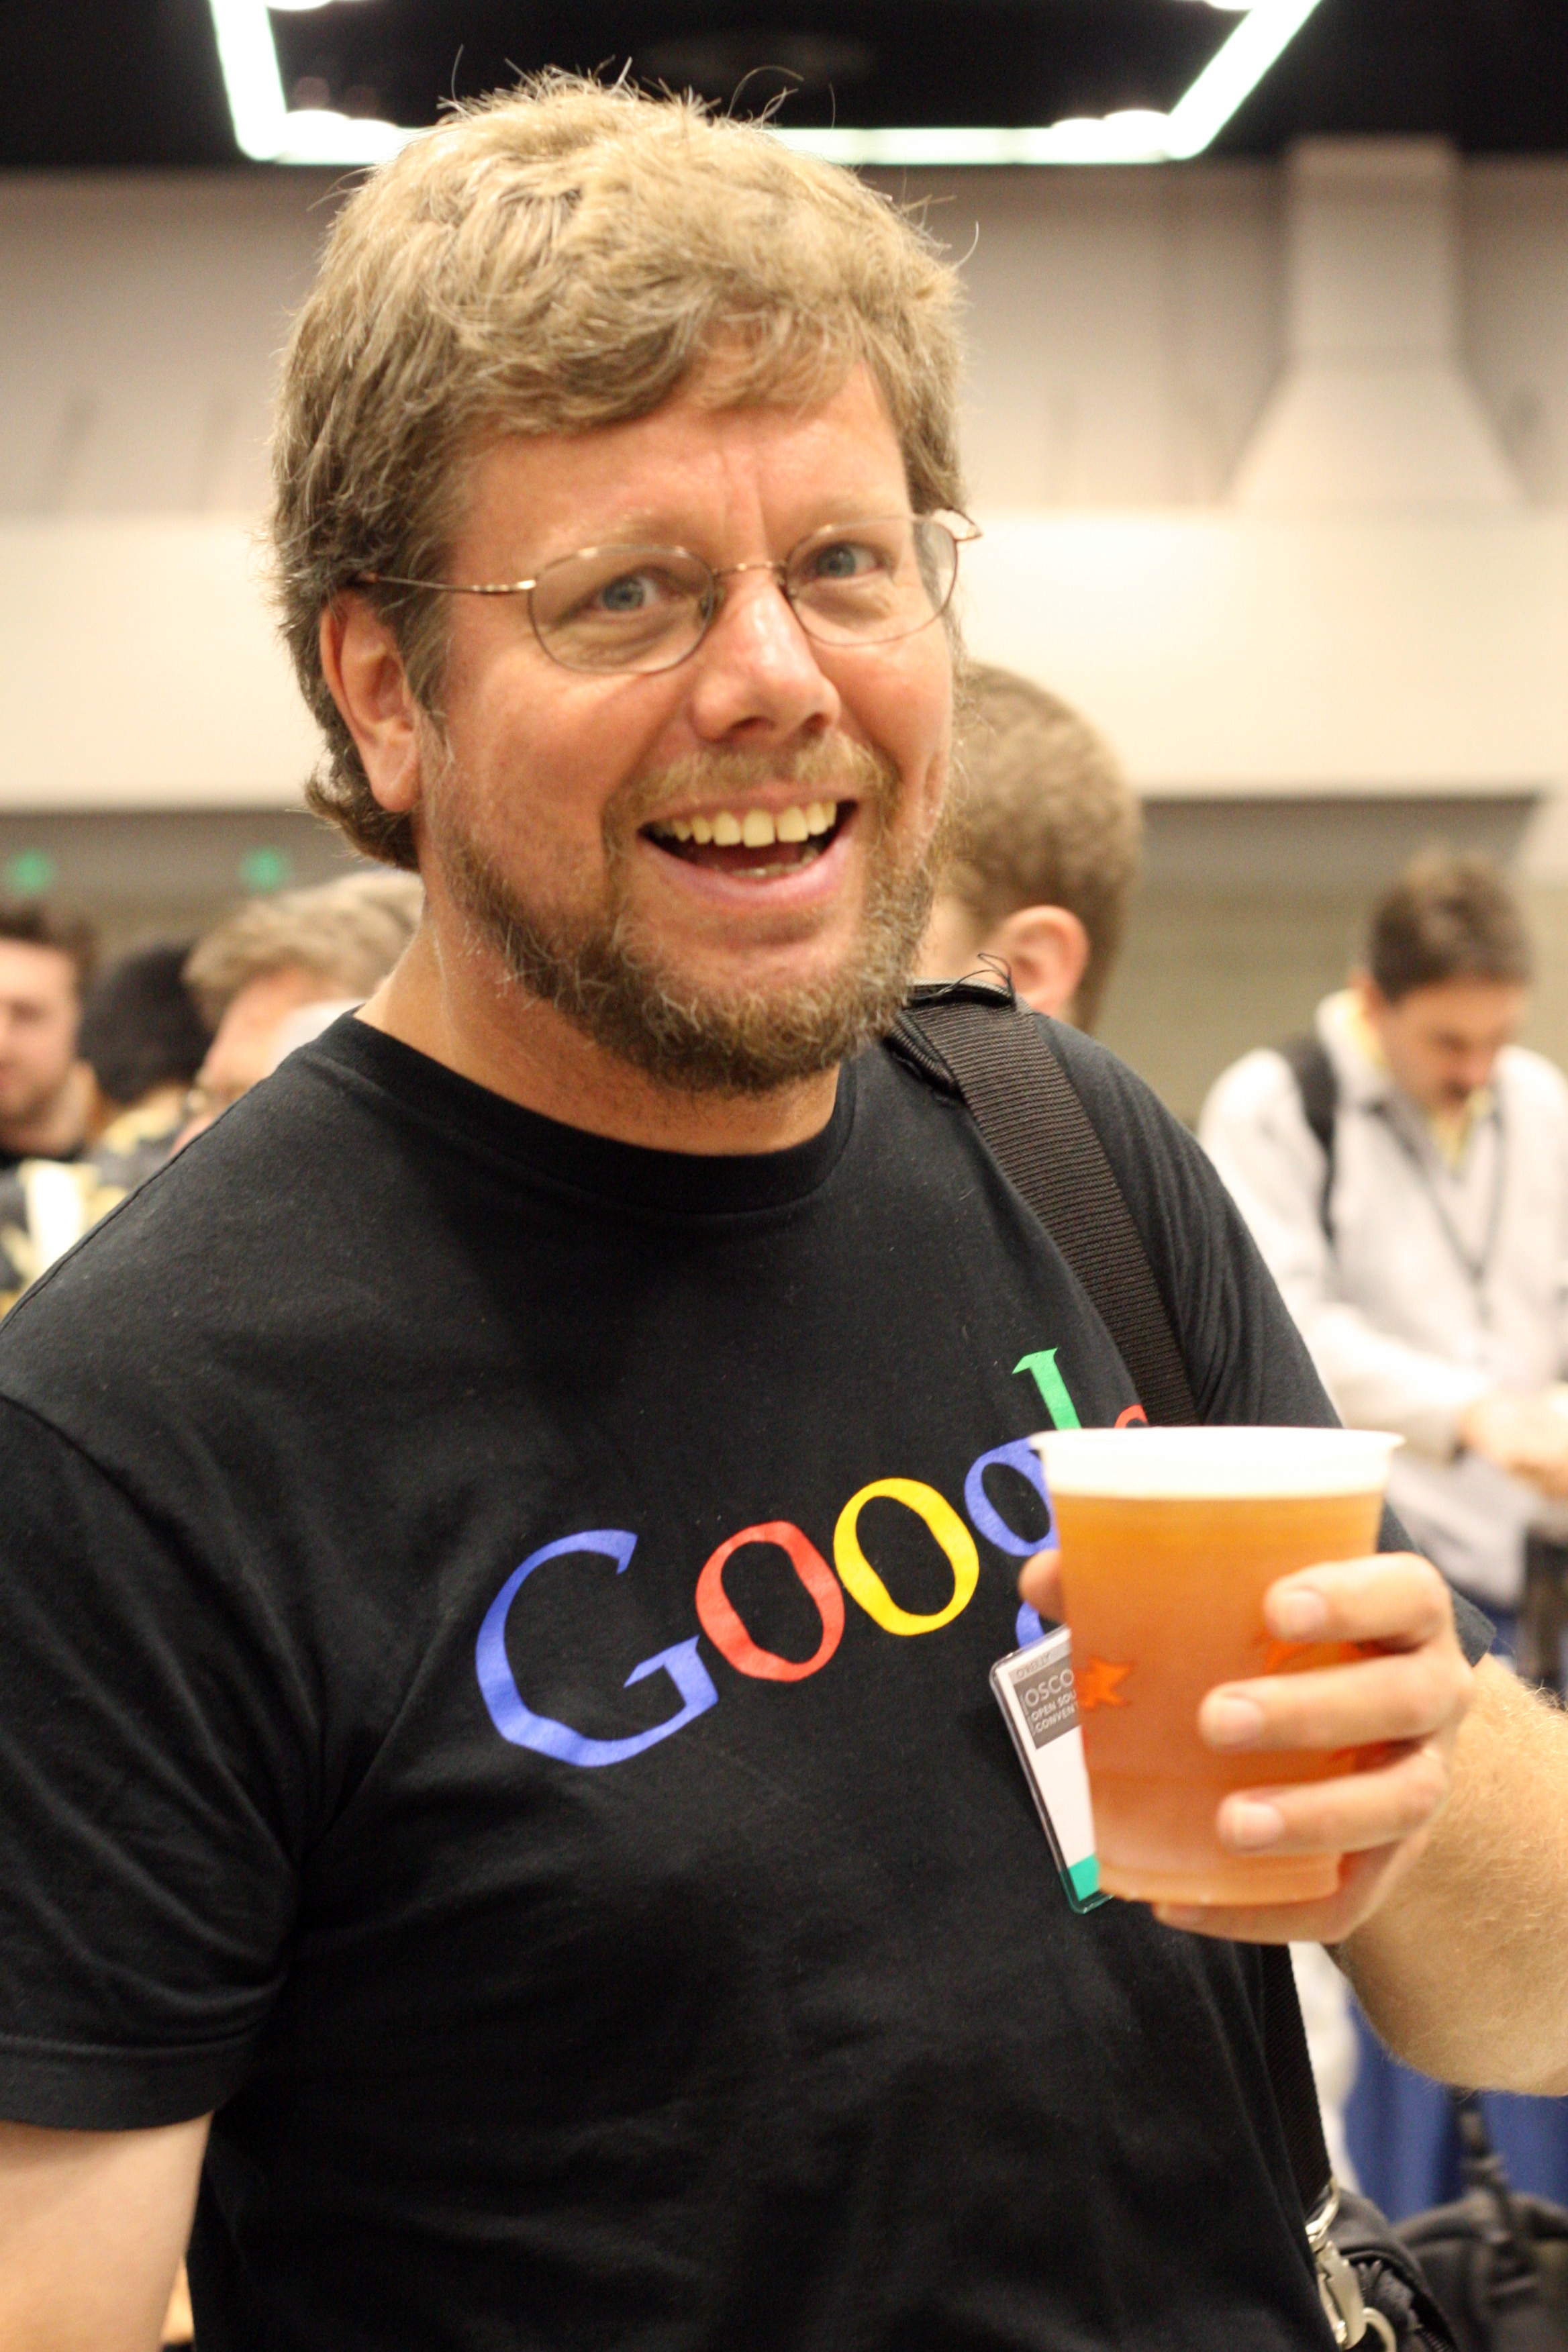
\includegraphics[width=0.4\textwidth]{fig/Guido_van_Rossum_OSCON_2006.jpg}
    \caption*{\centering\footnotesize{\color{gray}Guido Van Rossum at O'Reilly Open Source Convention, 2006, from Wikipédia}}
    \end{figure}
    \end{columns}
\end{frame}



\begin{frame}{Introduction}
    \framesubtitle{To be pythonic or not to be pythonic}
    % Zen of python
    \begin{block}{The Zen of Python, by Tim Peters}
        \begin{itemize}
        \item Beautiful is better than ugly.
        \item Explicit is better than implicit.
        \item Simple is better than complex.
        \item Complex is better than complicated.
        \item ...
        \end{itemize}
    \end{block}
    \centering
    \url{https://en.wikipedia.org/wiki/Zen_of_Python}
\end{frame}

\begin{frame}{Introduction}
    \framesubtitle{Python 101 \& Domaines d'utilisation}
    \begin{itemize}
        \item Langage de ``haut niveau''
        \item Langage multi-paradigmes (orienté objet, procédural, fonctionnel)
        \item Langage/syntaxe souple : grande variété d'utilisation
        \item Application web, Développement d'interfaces graphiques, etc.
        \item Interfaçage avec des langages plus complexes et performants (C, C++, Fortran, Rust, ...)
        \item Populaire (TIOBE index \#1)
        \item Platform independant (Windows, Linux, MacOS, etc.)
    \end{itemize}
\end{frame}

% ----------------------------------------------------------------
\section{Scientific Python ecosystem}
\begin{frame}{Ecosystème python scientifique}
    \framesubtitle{Et la science dans tout ça ?}
    \centering
    \begin{figure}
        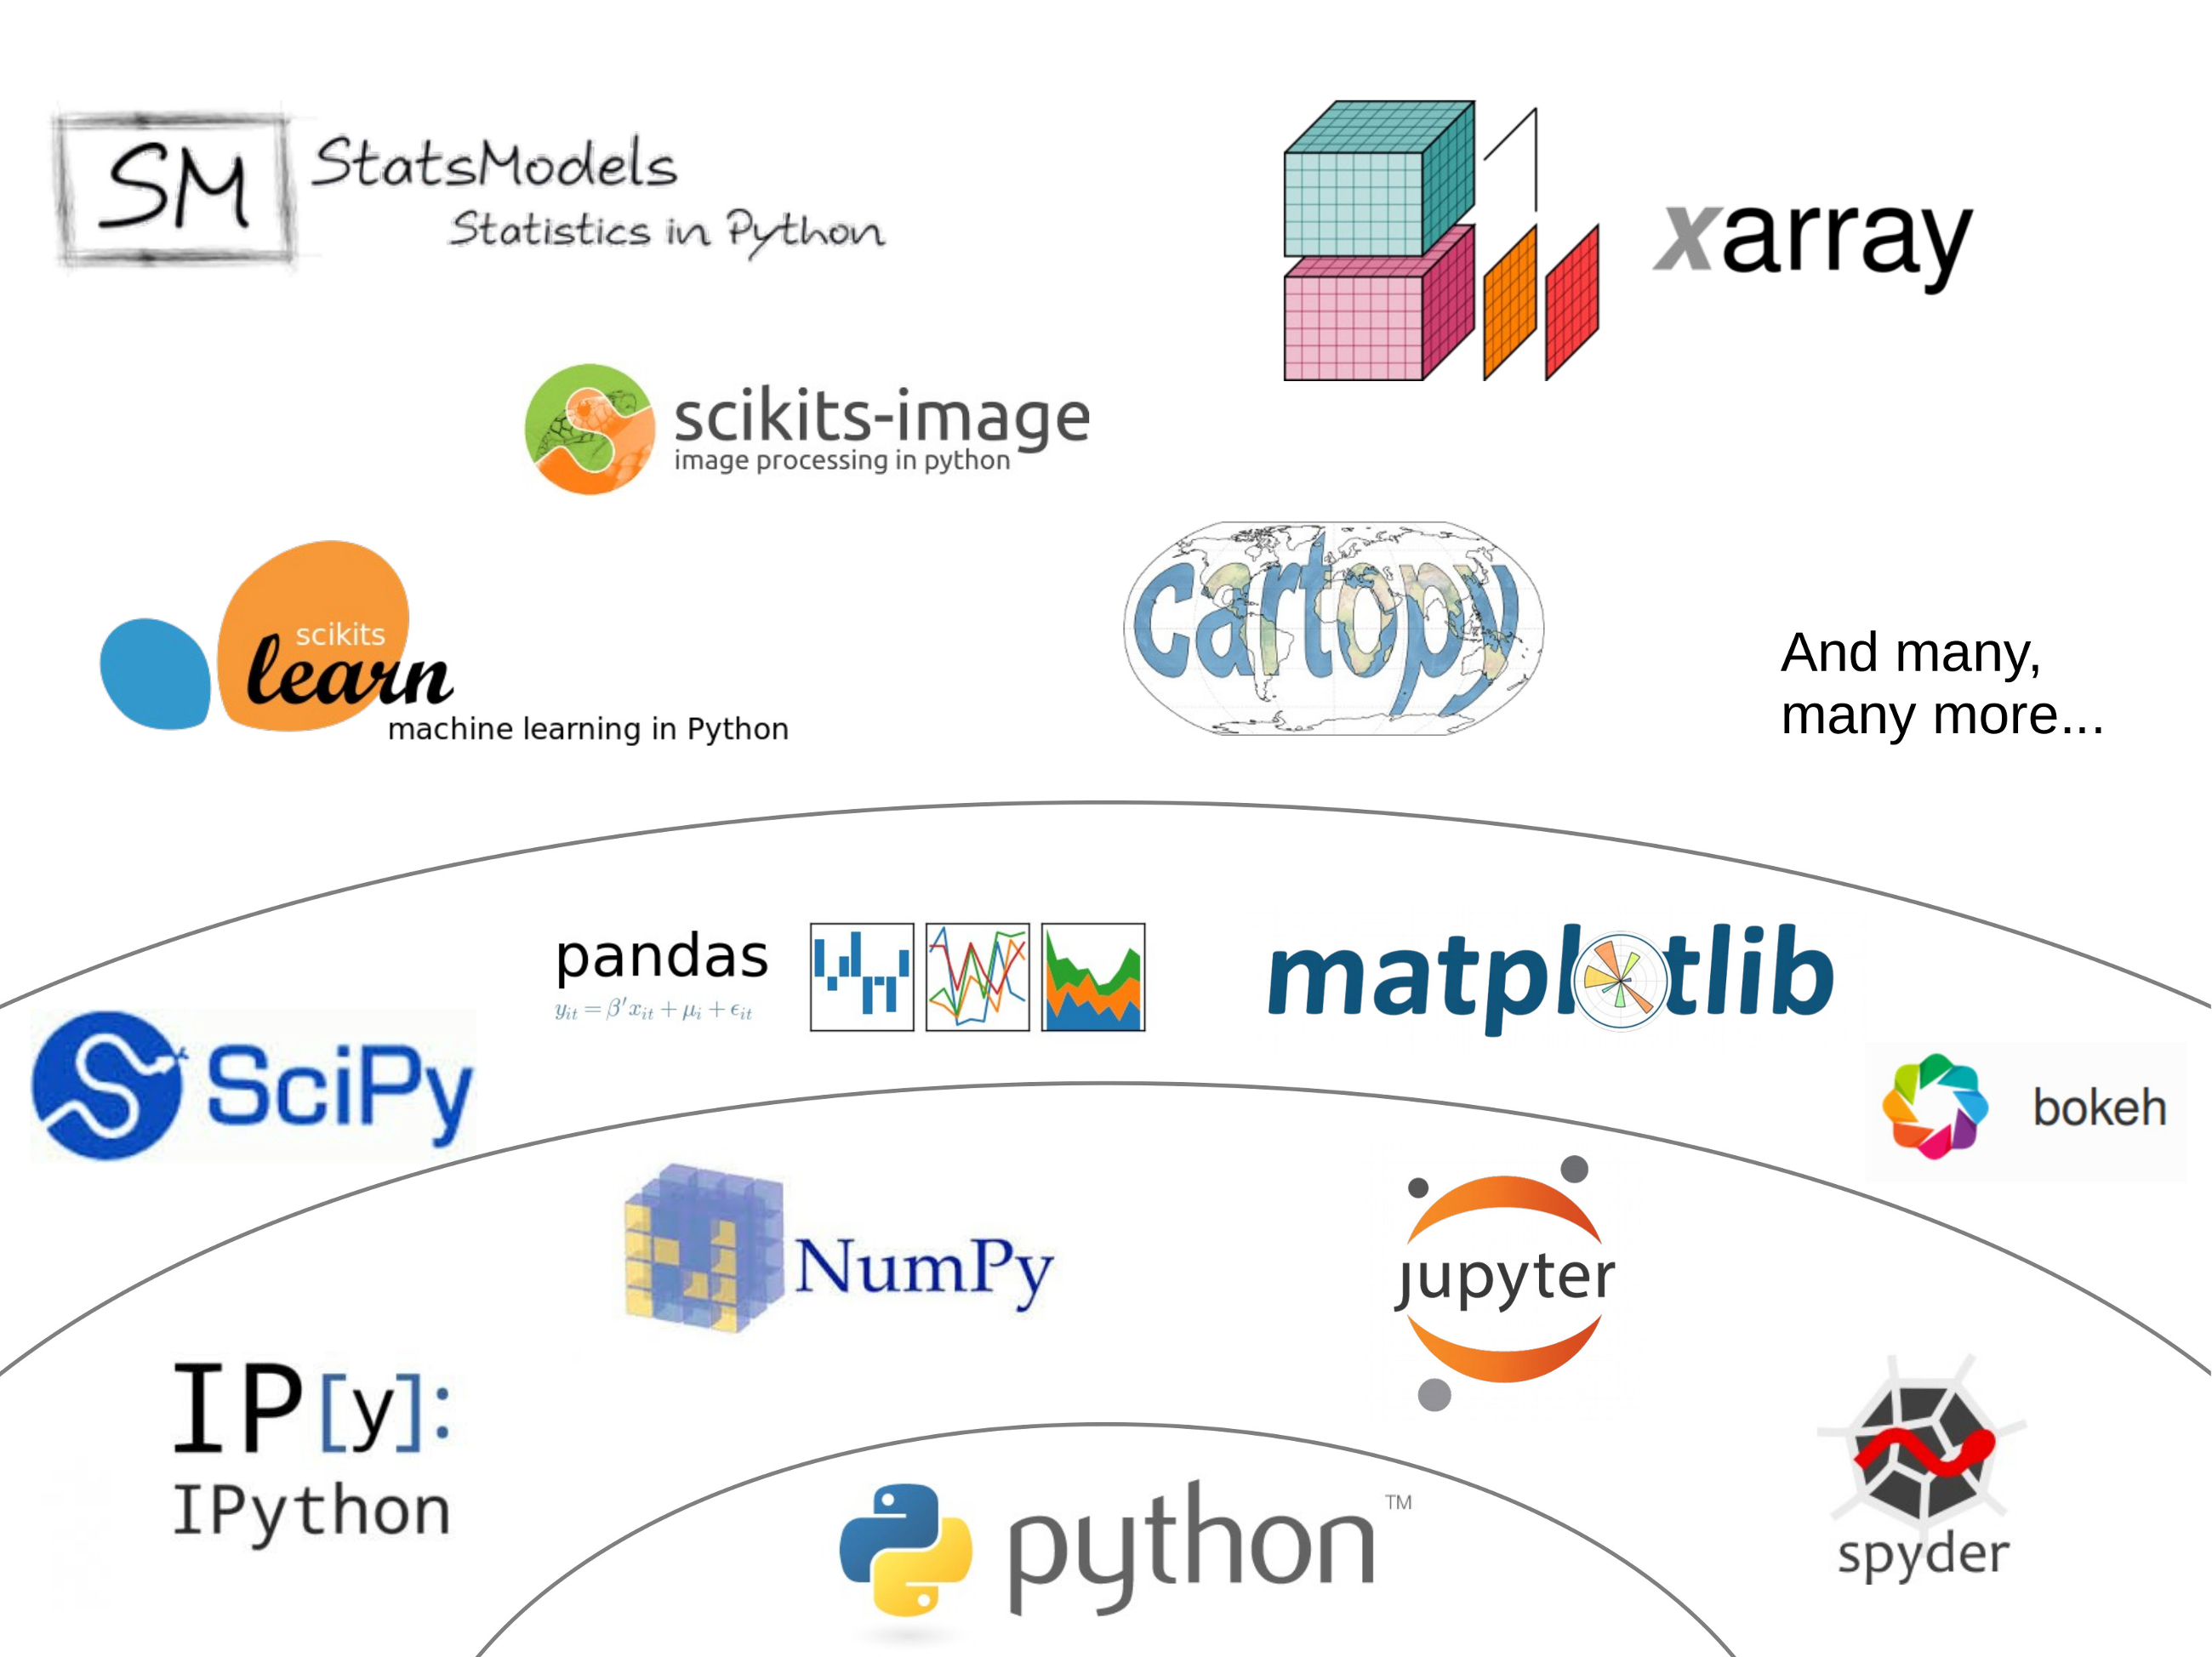
\includegraphics[scale=0.35]{fig/scipy_ecosystem.png}\\
        \caption*{\centering\footnotesize{\color{gray}
        Source: \url{https://fabienmaussion.info/scientific_programming/week_05/02-Scientific-Python.html}
        }}
    \end{figure}
\end{frame}

%---------------------------------------------
\section{More stuffs}

\begin{frame}{Installation}
    \framesubtitle{Distribution}
    \begin{columns}
    \column{0.6\textwidth}
    \small
    Installation:
    \begin{itemize}
        \item GNU/Linux: \texttt{python3} est intégré~;
        \item Windows: Installation de Cpython (\url{https://www.python.org/}) ou Distribution \texttt{conda}~;
    \end{itemize}

    Distribution:
    \begin{itemize}
        % TODO: expliciter conda env+package // pip que package, néc venv pour env
        \item Gestionnaire de paquet: \texttt{pip} (Python  Package Index) ou \texttt{conda} (conda-forge)
        \item gère l'installation de librairies tierces, voire les environnements virtuels
        \item les environnements virtuels permettent d'isoler les dépendances d'un projet à un autre (+ fichier pour reproduction)
        \item \texttt{conda} gère aussi des dépendances non python, mais est plus lourd à installer et à utiliser
        \item Mémo: ne plus utiliser Anaconda (Licence!)
    \end{itemize}
    \column{0.4\textwidth}
    \begin{tikzpicture}[remember picture, overlay]
    \node[anchor=center,yshift=2cm, xshift=-3cm, opacity=1] at (current page.east){ 
\includegraphics[width=0.4\linewidth]{fig/pypi.png}};
    \node[anchor=center,yshift=0.5cm, xshift=-1cm, opacity=1] at (current page.east){ 
\includegraphics[width=0.3\linewidth]{fig/conda}};
    \node[anchor=center,yshift=-2cm, xshift=-2.5cm, opacity=1] at (current page.east){ 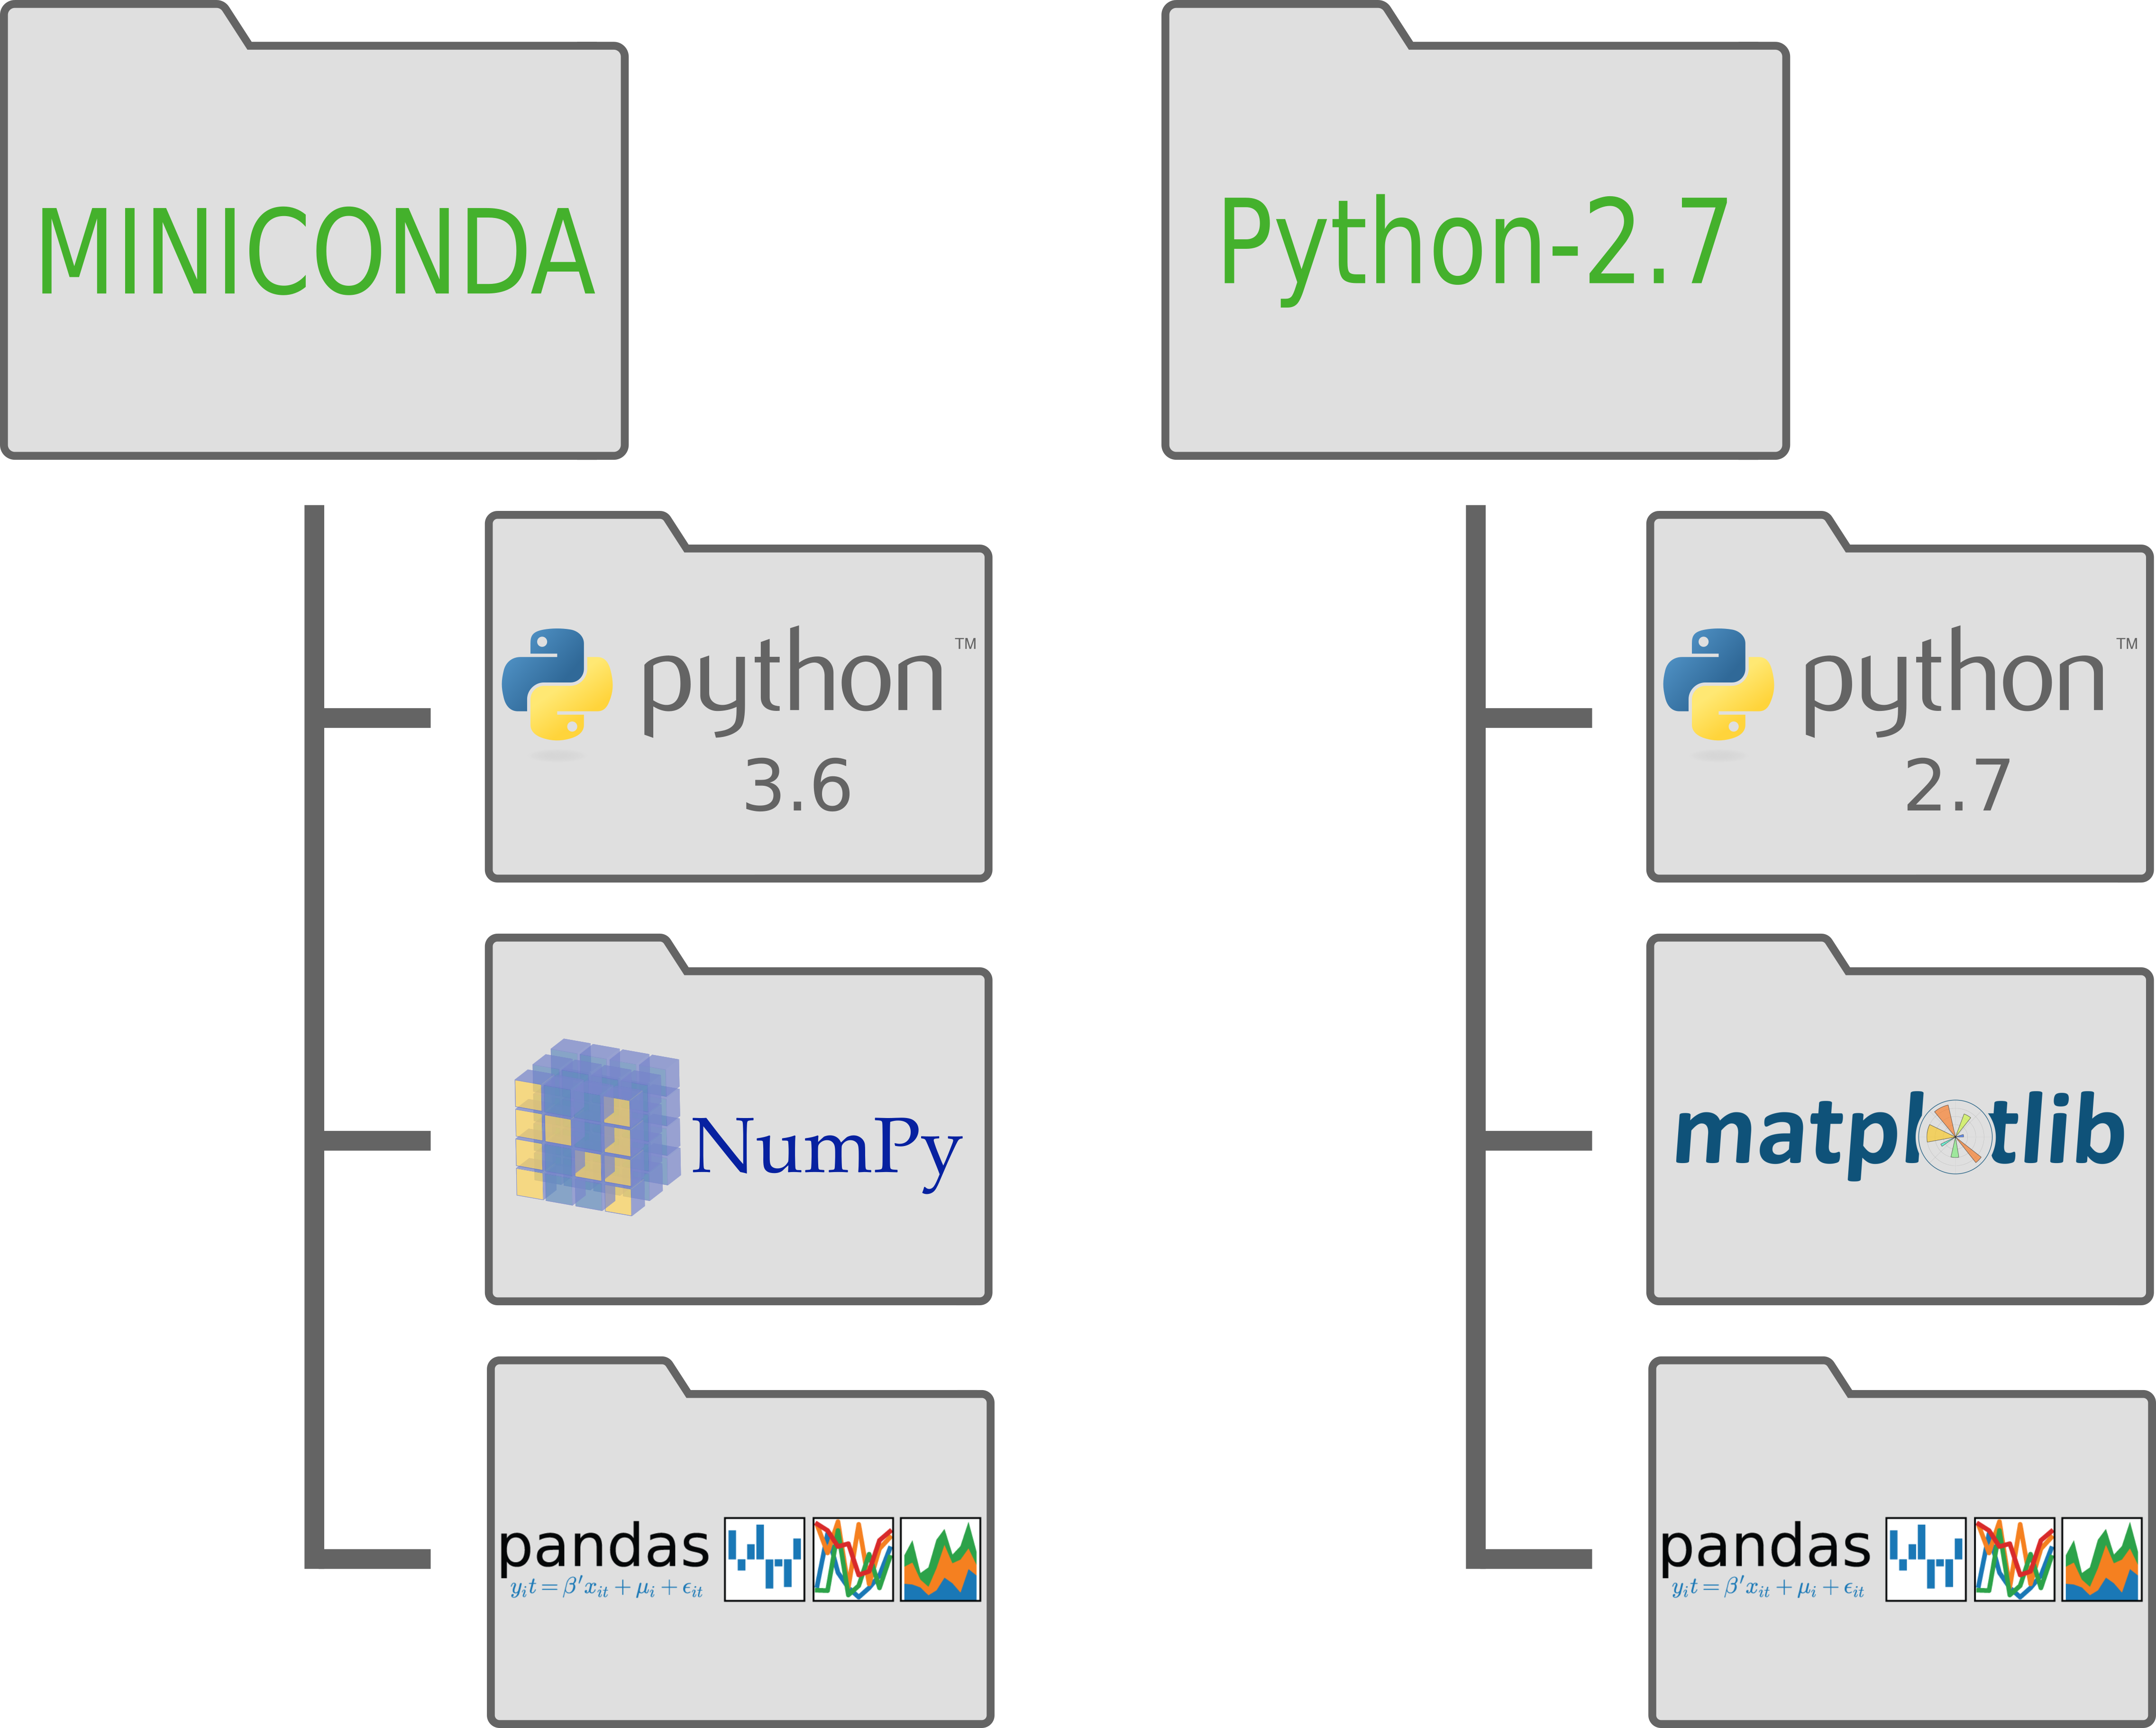
\includegraphics[width=0.5\linewidth]{fig/env.png}};
    \end{tikzpicture}
    \end{columns}
\end{frame}

\begin{frame}{Installation}
    \framesubtitle{Environnement de travail}
    \begin{columns}
    \column{0.6\textwidth}
    \begin{itemize}
        \item shell: \texttt{bash} (Linux) ou \texttt{powershell/cmd} (Windows)
        \item interpréteur python,
        \item éditeur de texte (vim, notepad, ...)
        \item IDE (Visual Studio Code, PyCharm, Spyder, ...)
        \item éventuellement: notebooks (Jupyter, VSCode, ...)
    \end{itemize}
    \column{0.4\textwidth}
    \begin{tikzpicture}[remember picture, overlay]
    \node[anchor=center,yshift=2cm, xshift=-3cm, opacity=1] at (current page.east){ 
\includegraphics[width=0.15\linewidth]{fig/bash}};
    \node[anchor=center,yshift=1.2cm, xshift=-1cm, opacity=1] at (current page.east){ 
\includegraphics[width=0.15\linewidth]{fig/vim}};
    \node[anchor=center,yshift=0.5cm, xshift=-3cm, opacity=1] at (current page.east){ 
\includegraphics[width=0.15\linewidth]{fig/code.jpg}};
    \node[anchor=center,yshift=-2cm, xshift=-3.5cm, opacity=1] at (current page.east){ 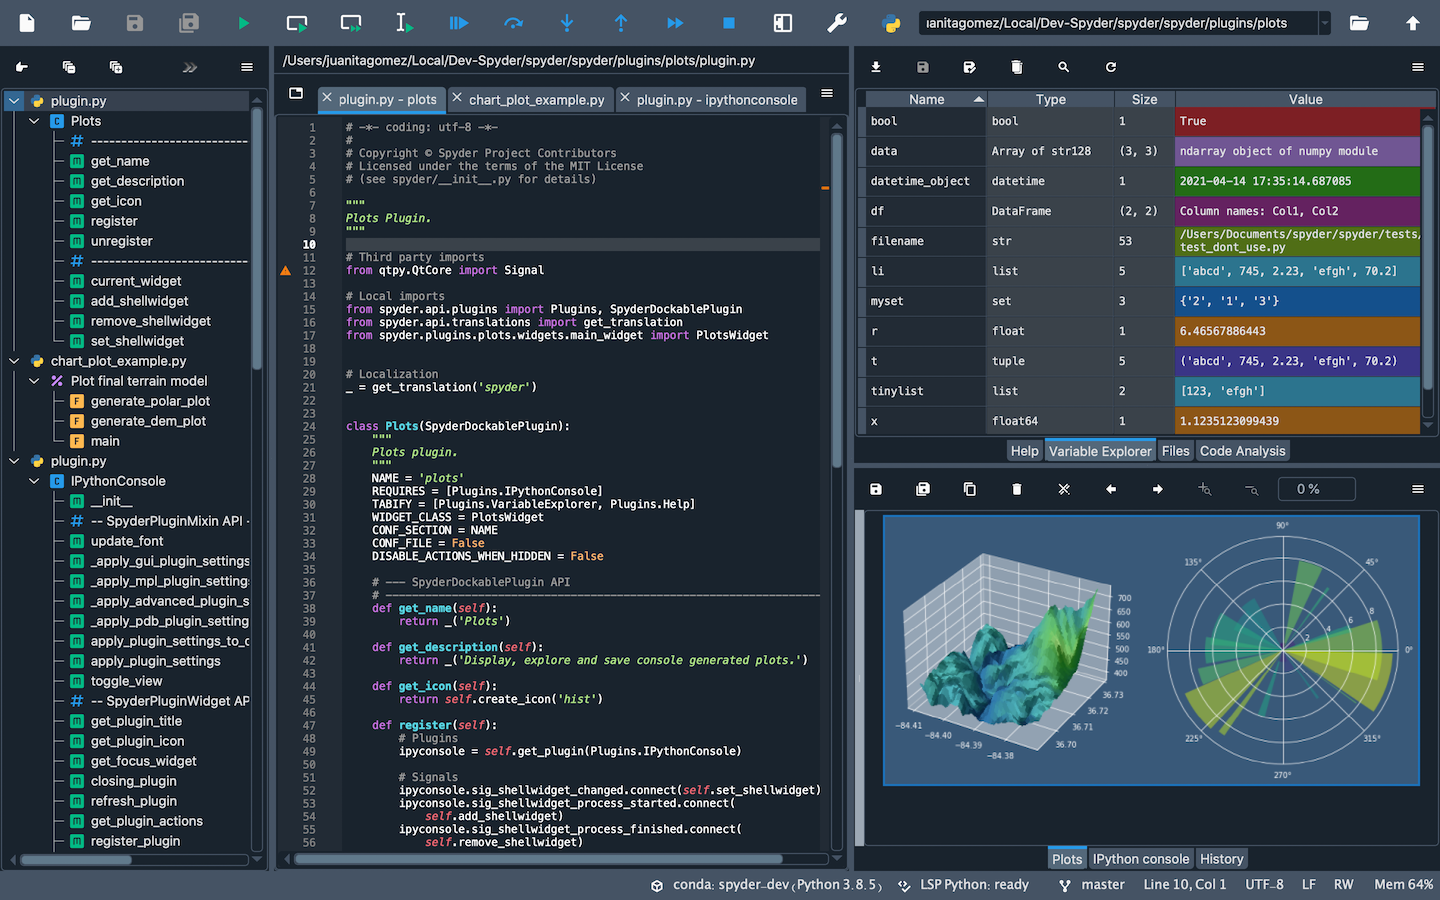
\includegraphics[width=0.9\linewidth]{fig/spyder}};
    \end{tikzpicture}
    \end{columns}
\end{frame}


\begin{frame}{Bonnes pratiques}
    \framesubtitle{En langue commune, ces signes disent...}
    
    La programmation incite à la rigueur et à des règles partagées pour la collaboration.\\
    
    Quelques bonnes pratiques informatiques peuvent être rappelées \parencite{speedOrganizingDataReproducible2023}
    
    \begin{itemize}
        \item structure de travail (arborescence, fichiers, ...) claire,
        \item documentation minimum (métadonnées, readme, ...)
        \item règles de base de nommage des fichiers/dossiers (pas d'espaces, pas de caractères spéciaux, ...),
        \item format de date, encodage: privilégier les standards (ISO 8601, UTF-8, ...)
        \item format de fichiers : standards et ouverts (csv, geopackage, netCDF, ...) // bannir Excel
    \end{itemize}
    
\end{frame}


\begin{frame}{Collaboration et code open-source}
    \framesubtitle{Partage, versionning de code source: Git}
    \begin{columns}
    \column{0.6\textwidth}
    \small
    \brieftitle{Outil vs. plateforme de collaboration}
    \begin{itemize}
        \item Git (outil) : Gestion de version (historique de révisions, release, ...),
        \item Plateforme : Partage de code source (github, gitlab, codeberg, ...),
        \item Collaboration (pull requests, issues/work items, ...),
    \end{itemize}
    \brieftitle{MAIS}
    \begin{itemize}
        \item outil expert (par des informaticiens, pour des informaticiens)
        \item Pas adapté au versionning de données, fichiers lourds, binaires, ...
        \item Quand on utilise un code open-source: attention aux licences (MIT, BSD, GPL, ...)
        et implications (copyleft) !
        \item Software provided ``AS IS'', no warranty, no support, no guarantee, no liability, ...
    \end{itemize}
    \column{0.4\textwidth}
    \centering
    
\includegraphics[width=0.2\textwidth]{fig/git}\\
    \vspace{0.5cm}
    
\includegraphics[width=0.4\textwidth]{fig/programmerhumor-io-programming-memes-e5afcbdde7eeb69} \\
    \vspace{1cm}
    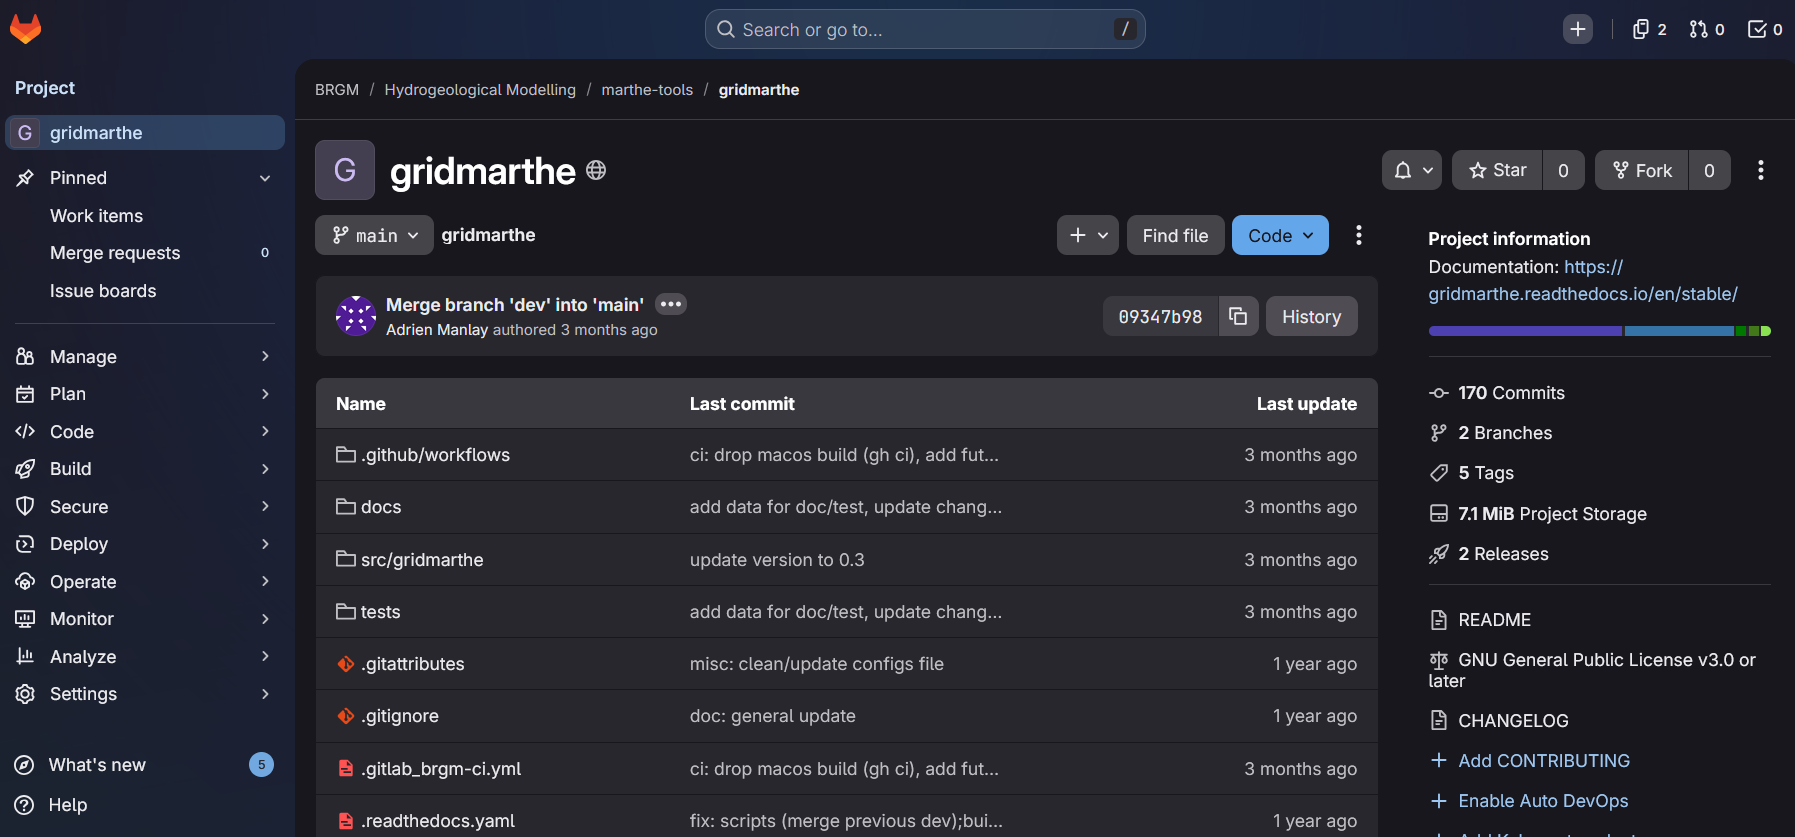
\includegraphics[width=\textwidth]{fig/gitlab}
    \end{columns}
\end{frame}


\begin{frame}{Quelques nuances sur Python}
    \framesubtitle{Pros \& Cons}
    
    \begin{columns}
    \column{0.7\textwidth}
    
    \brieftitle{Avantages de Python}
    \begin{itemize}
        \item Langage libre et ouvert
        \item Support gratuit disponible (la doc !, Stack Overflow, IA [?])
        \item bibliothèque standard, et bibliothèques tierces très riche
        \item Courbe d'apprentissage lente pour les fonctions très avancées, mais rapide pour les fonctions de base
    \end{itemize}
    
    \brieftitle{Faiblesses de Python}
    \begin{itemize}
        \item Pas de vérification statique du typage (ok, dis comme ça... mais ça peut être important!)
        % \item Pas de possibilité de générer de binaire compilé en natif
        \item Peu d'optimisation automatiques de la part de l'interpréteur:
        peu être lent...
        \item ``Easy to write bad code'', ``Straight way to disaster...''
    \end{itemize}
    
    \column{0.3\textwidth}
    \begin{tikzpicture}[remember picture, overlay]
    \node[anchor=center,yshift=2cm, xshift=-3cm, opacity=1] at (current page.east){ 
\includegraphics[width=0.4\linewidth]{fig/stack_bis}};
    \node[anchor=center,yshift=0.5cm, xshift=-1cm, opacity=1] at (current page.east){ 
\includegraphics[width=0.3\linewidth]{fig/rtfm}};
    \node[anchor=center,yshift=-2cm, xshift=-2cm, opacity=1] at (current page.east){ 
\includegraphics[width=0.6\linewidth]{fig/programmerhumor-io-programming-memes-04375dcda84c65d.jpg}};
    \end{tikzpicture}
    
    \end{columns}
\end{frame}

\section{Références}
\begin{frame}{Ressources complémentaires}
    \begin{itemize}
        \item Excellent MOOC sur Python 3:
    \url{https://www.fun-mooc.fr/en/cours/python-3-des-fondamentaux-aux-concepts-avances-du-langage/}
        \item Documentation officielle de Python:
    \url{https://docs.python.org/3/}
        \item Documentation officielle de la bibliothèque standard:
        \url{https://docs.python.org/3/library/index.html}
\end{itemize}
\end{frame}

%---------------------------------------------
{
% \setbeamertemplate{footline}{} % remove foot for titlepage
\begin{frame}[allowframebreaks,noframenumbering]{Références}
    \renewcommand*{\bibfont}{\footnotesize}
    \printbibliography[heading=none]
\end{frame}
}

\begin{frame}{Acknowledgement}
    Cette présentation est librement et fortement inspirée par celles de JP Vergnes, R. Aissat, (BRGM),
    M. Fienen (USGS). \\
    Les exercices qui suivent sont repris de la formation python BRGM, développée par
    Farid Smaï et Théophile Guillon.
\end{frame}


%---------------------------------------------
\appendix % end TOC
\setbeamertemplate{footline}{} % remove foot for titlepage
%---------------------------------------------
\section{End}
{
% \setbeamertemplate{footline}{}
\usebackgroundtemplate{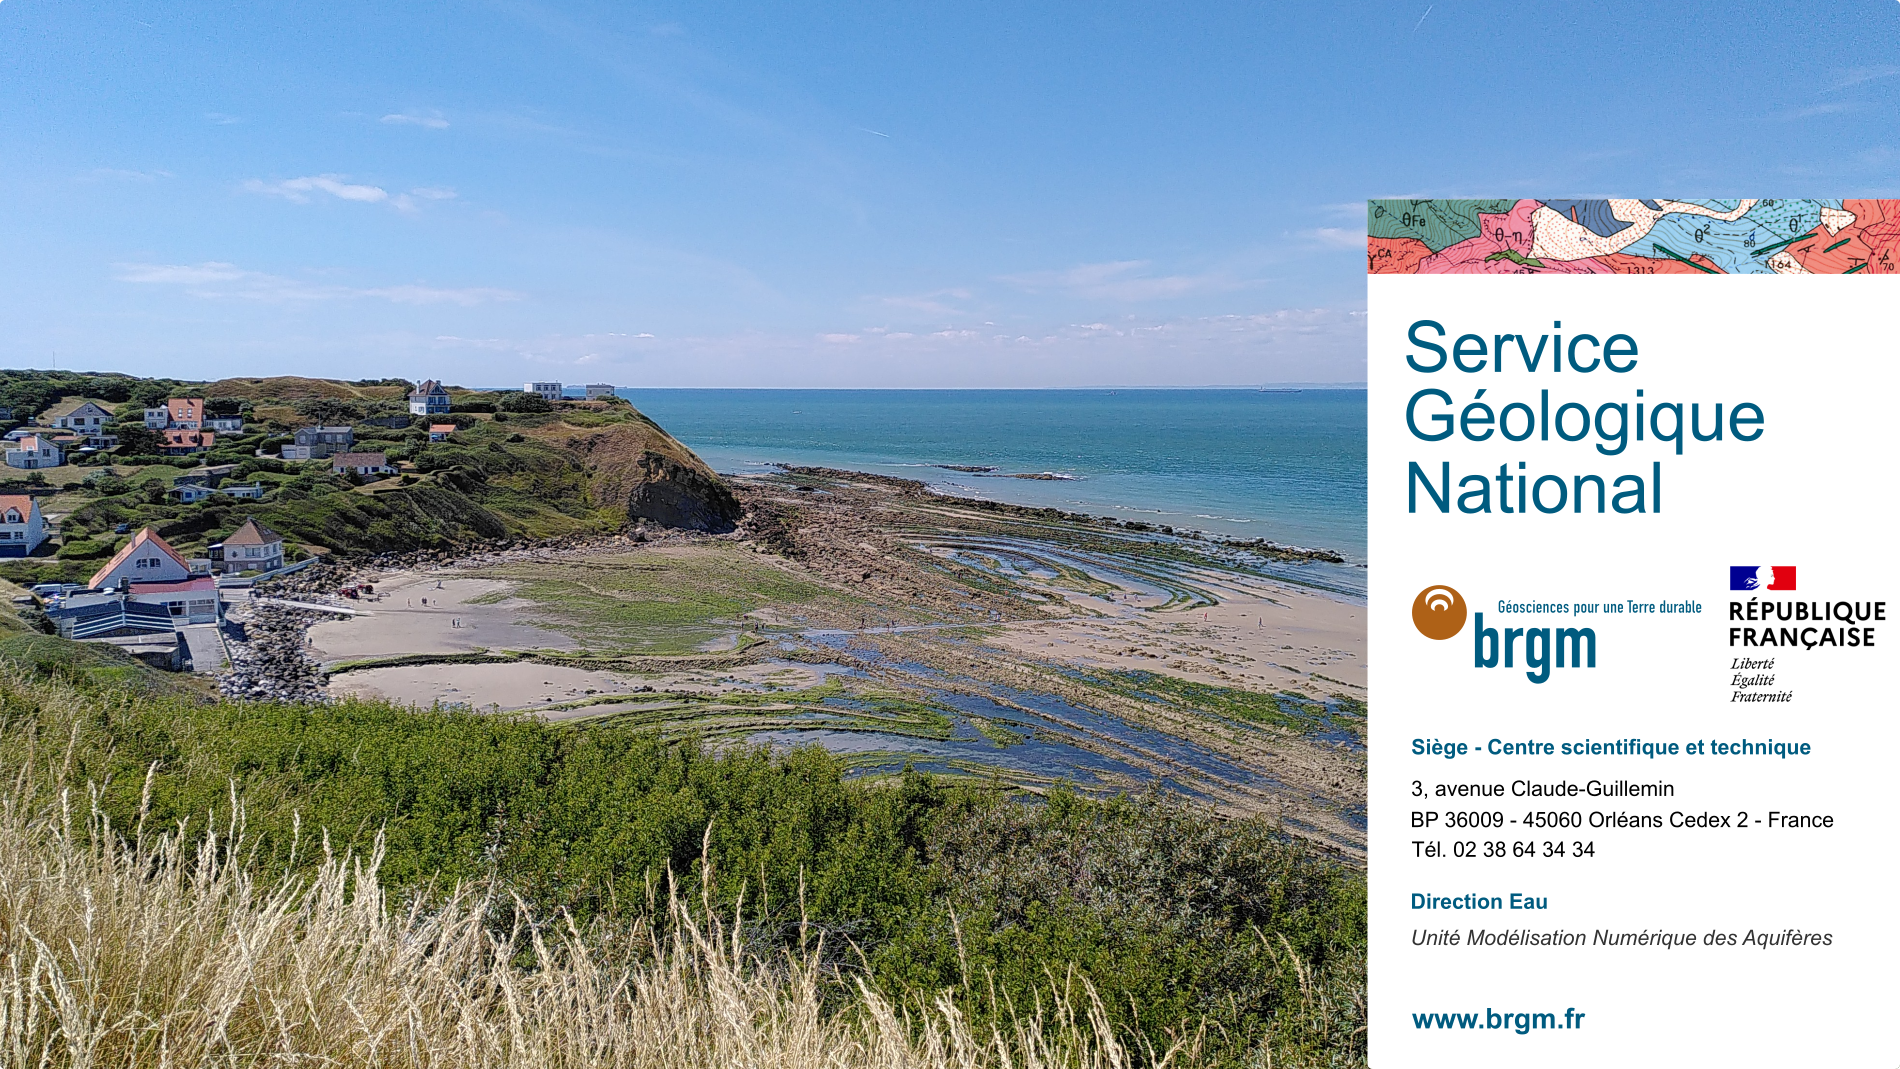
\includegraphics[width=\paperwidth, height=\paperheight]{beamertheme-brgm/back_cover.png}}
\begin{frame}[plain,noframenumbering]
    \begin{transbox}{0.5}  %ajoute la bande grise, si background par exemple
    \huge{\color{white} \textbf{Merci pour votre attention.\\
    \color{BrgmOrange}Des questions ?}}
    \end{transbox}
\end{frame}
}

\section{Extras}

% \begin{frame}[noframenumbering]
    % \frametitle{Impact de l'assimilation sur l'estimation du SPLI}
    % \framesubtitle{Analyse des séries temporelles simulées}
    % \begin{figure}[h]
    % \centering
    % \includegraphics[scale=0.2]{fig/spli/spli_00471X0010.png}
    % \includegraphics[scale=0.2]{fig/spli/spli_00636X0020.png}
    % \caption{Comparaison des indicateurs piézométriques standardisés
    % (SPLI) entre l'assimilation de données et le modèle sans assimilation}
    % \label{fig:spli_comparison}
% \end{figure}
% \end{frame}

\end{document}
% ============================================== %
